%!Tex Root = ../Linux_Installation.tex
% ./content_Linux_Installation/Packete
% ./content_Linux_Installation/Design
% ./content_Linux_Installation/Deklarationen
% ./content_Linux_Installation/Before_Installation
% ./content_Linux_Installation/After_Base_Installation

\section{Ubuntu Base Installation}

\begin{frame}[fragile]{Ubuntu Manuelle Partitionierung}
  \begin{itemize}
    \item
  \end{itemize}
  % https://medium.com/linuxforeveryone/how-to-install-ubuntu-20-04-and-dual-boot-alongside-windows-10-323a85271a73
\end{frame}

\section{Arch Linux Base Installation}

\begin{frame}[fragile]{Nützliche Webseiten}
  \begin{itemize}
    \item \alert{Official Installation Guide:} \url{https://wiki.archlinux.org/title/Installation_guide}.
    \item \alert{Wichtige Meldungen:} \url{https://archlinux.org/}
  \end{itemize}
\end{frame}

\begin{frame}[fragile]{Keyboard Layout (for the Installation)}
  \begin{itemize}
    \item \inlinebox*{ls /usr/share/kbd/keymaps/**/*.map.gz | less}
    \begin{figure}
      
\includegraphics[width=0.5\textwidth]{./figures/keyboard.png}
    \end{figure}
    \item \inlinebox*{loadkeys de-latin1-nodeadkeys}
  \end{itemize}
\end{frame}

\begin{frame}[fragile,allowframebreaks]{Wifi connection\vspace{0.25cm}}
  \begin{itemize}
    \item \inlinebox*{ping -c 1 google.com}
    \begin{itemize}
      \item \alert{if not:} $\Rightarrow$ Boxes
    \end{itemize}
    \begin{block}{LAN}
      \begin{itemize}
        \item \alert{find out interface:} \inlinebox*{ip link} or \inlinebox*{ip a} (\inlinebox{addr show}).
          \begin{itemize}
            \item ignore loopback.
          \end{itemize}
        \item \inlinebox{ip link set dev <interface-name>}.
        \item \inlinebox{dhcpcd enp1s0 <interface-name>}.
      \end{itemize}
    \end{block}
    \begin{block}{WLAN}
      \begin{itemize}
        \item Shell öffnen: \inlinebox{iwctl} (\inlinebox{sudo pacman -S iwd}), \inlinebox{systemctl enable iwd.service --now}.
        \item \alert{wireless interfances installed on system:} \inlinebox{device list}.
        \item \alert{start search for wireless access points:} {\tiny \inlinebox{station <name of device, e.g. wlan0> scan}}.
        \item \alert{found wifi networks:} {\tiny\inlinebox{station <name of device, e.g. wlan0> get-networks}.}
        \item \alert{connect:} {\tiny \inlinebox{station <name of device, e.g. wlan0> connect "<name of network>"}.}
        \item \alert{disconnect from prompt:} \key{Ctrl-d}.
        \item \alert{check if all worked:} \inlinebox{ip addr show} if it shows a ip address.
      \end{itemize}
    \end{block}
  \end{itemize}
  % \begin{Sidenote}
  %   \begin{itemize}
  %     \scriptsize
  %     \item sometimes one has to manually start the dhcp client \inlinebox{dhcpcd}.
  %     \item netctl (and therefore wifi-menu) got removed from the Arch Linux ISO starting July 2020. To get connected while installing Arch, use \inlinebox{iwctl}. If it's blocked, either use that physical switch, or use \inlinebox{rfkill unblock wifi}. Then, type in \inlinebox{iwctl}. When you're in \inlinebox{iwctl}, use \inlinebox{device list} to see the name that the wifi router is using. For commands after this, replace device with the name of the device as found using the \inlinebox{device list} command. If you want to get the name of the network you want to use, use \inlinebox{station device scan} and then \inlinebox{station device get-networks}. After that, type in \inlinebox{station device connect SSID*}, with the *SSID being the name of the internet you want to use. If there is a password on the wifi, type that in when it asks for the wifi. After that, press Ctrl+C to get back to the terminal/root@archiso.
  %   \end{itemize}
  % \end{Sidenote}
\end{frame}

\begin{frame}[fragile]{Check UEFI}
  \begin{itemize}
    \item \alert{check for uefi mode:} \inlinebox{ls /sys/firmware/efi/efivars} check if exists.
      \begin{itemize}
        \item There should be output.
      \end{itemize}
  \end{itemize}
\end{frame}

\begin{frame}[fragile]{Reorder Mirrorlist (optional)}
  \begin{itemize}
    \item \alert{reorder mirrolist:} \inlinebox{nvim /etc/pacman.d/mirrorlist} (first entry will be taken first, if offline the second etc.)
    \item \inlinebox{/usr/bin/rankmirrors}
    \item \url{https://archlinux.org/mirrors/status/}
  \end{itemize}
\end{frame}

\begin{frame}[fragile, allowframebreaks]{Partitioning\vspace{0.5cm}}
  \begin{itemize}
    \item \inlinebox{lsblk -f}, \inlinebox{fdisk -l | more} or \inlinebox{df -h}, \inlinebox{mount} (for currently mounted filesystem)
    \item \inlinebox{cfdisk /dev/sda}
    \item \inlinebox{gpt}, enter
    \item move with arrow keys to \inlinebox{New}, enter, type \inlinebox{512M}, enter (efi-partition)
    \item select \inlinebox{Type}, \inlinebox{EFI-System}
    \item move down to next Free space and next \inlinebox{2G} (swap-partition)
    \item select \inlinebox{Type}, \inlinebox{Linux swap}
    \item next \inlinebox{20G} (root-Partition)
    \item for floating number: \inlinebox{17.5G}
    \item it's type is automatically \inlinebox{Linux filesytem}
    \item next e.g. \inlinebox{80G} (home-Partition)
    \item it's type is automatically \inlinebox{Linux filesytem}
    \item move to \inlinebox{Write} and answer \inlinebox{yes} (enter doesn't write anything)
    \item move to \inlinebox{Quit}
    \item (\inlinebox{fdisk} is the old way)
    \item \inlinebox{mkfs.fat -F32 /dev/sda1}
    \item \inlinebox{mkswap /dev/sda2}
    \item \inlinebox{swapon /dev/sda2}
    \item \inlinebox{mkfs.ext4 /dev/sda3} and \inlinebox{mkfs.ext4 dev/sda4}
  \end{itemize}
\end{frame}

\begin{frame}[fragile, allowframebreaks]{Install to Partition\vspace{0.5cm}}
  \begin{itemize}
    \item \inlinebox{mount /dev/sda3 /mnt}
    \item \inlinebox{mkdir /mnt/home}
    \item \inlinebox{mount /dev/sda4 /mnt/home}
    \item check mounting points with \inlinebox{lsblk}
    \item \inlinebox{pacstrap /mnt base linux linux-firmware}
      \begin{Sidenote}
        \begin{itemize}
          \scriptsize
          \item \inlinebox{linux-firmware} is required in order that the  wifi adapter will be automatically recognized after installation is completed
          \item install linux kernels: \inlinebox{pacman -S linux linux-headers linux-lts linux-lts-headers} (long term support kernel to have the possibility to choose if the other one stops working
          \item all installed previously has to be installed again, because it was only in the installation media
        \end{itemize}
      \end{Sidenote}
    \item \inlinebox{genfstab -U /mnt >> /mnt/etc/fstab} (generate filesystem table file) // vielleicht besser vor pacstrap?
    \item \inlinebox{cat /mnt/etc/fstab} (take a look at it)
      \item other options: \inlinebox{-p} and \inlinebox{-h} (help)
      \item \inlinebox{arch-chroot /mnt} (change into root directory of new installation, now root user in new linux system)
  \end{itemize}
  \begin{Sidenote}
    \begin{itemize}
      \scriptsize
      \item create ramdisk for the linux kernel: \inlinebox{mkinitcpio -p linux}, \inlinebox{mkinitcpio -p linux-lts} (or \inlinebox{-P})
    \end{itemize}
  \end{Sidenote}
\end{frame}

\begin{frame}[fragile,allowframebreaks]{Timezone\vspace{0.5cm}}
  \begin{itemize}
    \item \inlinebox{ln -sf /usr/share/zoneinfo/Europe/Berlin /etc/localtime} (use \inlinebox{tab} to see possible options)
    \item \inlinebox{vim /etc/locale.gen}, uncomment locale \inlinebox{en_US.UTF-8 UTF-8}
      \begin{itemize}
        \item determines the language, monetary values, time and date formats etc. of the system
        \item \inlinebox{pacman -S neovim}
      \end{itemize}
    \item \inlinebox{locale-gen} to generate the choosen locale
    \item \inlinebox{echo LANG=en_US.UTF-8 > /etc/locale.conf}
  \end{itemize}
\end{frame}

\begin{frame}[fragile,allowframebreaks]{Timezone}{timedatectl\vspace{0.5cm}}
  \begin{itemize}
    \item \inlinebox{timedatectl set-ntp true}: Controls whether network time synchronization is active and enabled (if available). If the argument is true, this enables and starts the first existing network synchronization service
      \begin{Sidenote}
        \begin{itemize}
          \item \alert{old way:} \inlinebox{sudo ntpd -qg} to manually synchronize your clock with the network, ignoring large deviations between local UTC and network UTC
        \end{itemize}
      \end{Sidenote}
    \item  \inlinebox{timedatectl set-timezone Europe/Berlin}: Set the system time zone to the specified value
      \item this will create an \inlinebox{/etc/localtime} symlink that points to a zoneinfo file under \inlinebox{/usr/share/zoneinfo/}
    \item \inlinebox{timedatectl list-timezones}: list available time zones
    \item \inlinebox{timedatectl set-time [TIME]}: set the system clock to the specified time. This will also update the RTC time accordingly. The time may be specified in the format "2012-10-30 18:17:16".
    \item \inlinebox{timedatectl}: check the current \alert{system clock} time (presented both in local time and UTC) as well as the RTC (\alert{hardware clock})
    \item there are two time standards: localtime and Coordinated Universal Time (UTC). The localtime standard is dependent on the current time zone, while UTC is the global time standard and is independent of time zone values
    \item the standard used by the hardware clock (CMOS clock, the BIOS time) is set by the operating system. By default, Windows uses localtime
    \item an OS that uses the UTC standard will generally consider the hardware clock as UTC and make an adjustment to it to set the OS time at boot according to the time zone
  \end{itemize}
\end{frame}

\begin{frame}[fragile,allowframebreaks]{Time}
  \begin{itemize}
    \item \inlinebox{timedatectl set-ntp true}
    \item verify with \inlinebox{timedatectl status} (or \inlinebox{date}), should be utc
    \item \inlinebox{hwclock --systohc --utc}: write the current software UTC time to the hardware clock
      \begin{itemize}
        \item If you specify neither \inlinebox{--utc} nor \inlinebox{--localtime} then the one last given with a set function  (\inlinebox{--set}, \inlinebox{--systohc}, or \inlinebox{--adjust}), as recorded in \inlinebox{/etc/adjtime}, will be used. If the adjtime file doesn't exist, the default is UTC
          \begin{itemize}
            \item the \inlinebox{date} time should correspond to current localtime
          \end{itemize}
        \item \inlinebox{sudo hwclock --show} (does already add up the winter time (+1) and the summer time (+2))
      \end{itemize}
    \item \inlinebox{systemctl enable systemd-timeyncd}
  \end{itemize}
\end{frame}

\begin{frame}[fragile,allowframebreaks]{User and Root}
  \begin{itemize}
    \item \inlinebox{echo ArchPC > /etc/hostname}, type in username
    \item \inlinebox{passwd} for root user
    \item \inlinebox{useradd -m -g users -G wheel areo} or \inlinebox{useradd -m -G users,wheel areo}
      \begin{itemize}
        \item or {\tiny\inlinebox{sudo useradd -m (-g username) -G additional_groups -s login_shell username}} or \inlinebox{useradd -n areo} and \inlinebox{usermod -aG wheel.audio.video.optical.storage areo}
        \item other options: \inlinebox{-s /bin/bash}
      \end{itemize}
    \item \inlinebox{passwd areo}
    \item \inlinebox{pacman -S sudo}
      \begin{itemize}
        \item find out if it's installed with \inlinebox{which sudo}
        \item else \inlinebox{pacman -S which sudo} or just directly \inlinebox{pacman -S base-devel}
      \end{itemize}
    \item \inlinebox{EDITOR=nvim visudo} to edit sudoers file in nvim and uncomment \inlinebox{%wheel ALL=(ALL) ALL}
    \item
  \end{itemize}
    \begin{Sidenote}
      \begin{itemize}
        \item user, group and password management tools on Arch Linux come from the shadow package, which is a dependency of the base package
      \end{itemize}
    \end{Sidenote}
  \begin{itemize}
      \item \inlinebox{hostnamectl set-hostname <hostname>}
    \begin{itemize}
      \item \inlinebox{cat /etc/hostname}
    \end{itemize}
    \item \inlinebox{nvim /etc/hosts} and add \inlinebox{127.0.0.1 localhost} and newline \inlinebox{127.0.1.1 <hostname>}
    \item check by running \inlinebox*{hostnamectl}
  \end{itemize}
\end{frame}

\begin{frame}[fragile,allowframebreaks]{Keyboard-Layout}
  \begin{itemize}
    \item \inlinebox{echo KEYMAP=de-latin1-nodeadkeys > /etc/vconsole.conf}
      \begin{itemize}
        \item for the tty, but no in X
      \end{itemize}
  \end{itemize}
\end{frame}

\begin{frame}[fragile,allowframebreaks]{Network}
  \begin{itemize}
     \item \inlinebox{nvim /etc/hosts}:
       \begin{terminal}[]
        # blablabla
        # blablabla

        127.0.0.1 localhost
        ::1 localhost
        127.0.1.1 ArchPC.localdomain ArchPC
     \end{terminal}
    \item \inlinebox{pacman -S networkmanager}
    \item \inlinebox{systemctl enable NetworkManager} (create symlink)
    \item \inlinebox{nm-applet}: symbol in systray to configure and have easy access to NetworkManager (\inlinebox{sudo pacman -S network-manager-applet})
      \begin{itemize}
      \item put \inlinebox{nm-applet &} into \inlinebox{~/.xinitrc}
      \item there's a autostart desktop entry automaticaly created under \inlinebox{/etc/xdg/autostart/nm-applet.desktop}
      \item i3 already autostarts it in it's \inlinebox{~/.configs/i3/config}: \inlinebox{exec --no-startup-id nm-applet}
      \end{itemize}
  \end{itemize}
  \begin{Sidenote}
    \begin{itemize}
      \item there is also \inlinebox{yay -S networkmanager-dmenu-git}.
    \end{itemize}
  \end{Sidenote}
  \begin{Sidenote}
    \begin{itemize}
      \item \alert{other packages:} \inlinebox{pacman -S wpa_supplicant wireless_tools netctl}, if there's no wired connection one can use \inlinebox{iwdctl} from the \inlinebox{iwd} package (earlier versions: \inlinebox{wifi-menu} from the \inlinebox{netctl} package).
    \end{itemize}
  \end{Sidenote}
\end{frame}

\begin{frame}[fragile,allowframebreaks]{Grub}
  \begin{itemize}
    \item \inlinebox{pacman -S grub efbootmgr dosfstools os-prober mtools}
    \item \inlinebox{mkdir /boot/EFI}
    \item \inlinebox{mount /dev/sda1 /boot/EFI}
    \item \inlinebox{grub-install --target=x86_64-efi --bootloader-id=OSName}
      \begin{itemize}
        \item \inlinebox{x86_64-efi} is for x86_64 systems
        \item other options: \inlinebox{--efi-directory=/boot/EFI --removable} or \inlinebox{--bootloader-id=GRUB} (bootloader identifier, here named GRUB. A directory of that name will be created in \inlinebox{esp/EFI/} to store the EFI binary and this is the name that will appear in the UEFI boot menu to identify the GRUB boot entry)
        \item by default the generation scripts automatically add menu entries for all installed Arch Linux kernels to the generated configuration. After installing or removing a kernel, you just need to re-run the above grub-mkconfig command
      \end{itemize}
      \begin{Sidenote}
        \begin{itemize}
          \scriptsize
          \item \inlinebox{mkdir /boot/grub/locale} and then 
\includegraphics[height=0.3cm]{./figures/cp.png} is propably not rly needed
          \item \inlinebox{--recheck} propably not rly needed
        \end{itemize}
      \end{Sidenote}
    \item \alert{Dualbooot with Windows:}
      \begin{itemize}
        \item use the EFI-Partition from Windows: \inlinebox{mount /dev/sda1 /boot/EFI}
        \item if two EFI-Partitions exist (one from Windows: \inlinebox{/dev/sda1}  and one for Arch: \inlinebox{dev/sda5}): \inlinebox{mount /dev/sda1/ /mnt} (EFI-Partition of Windows has to be mounted, so that the os-prober can find it) or \inlinebox{mdkdir /mnt2} and \inlinebox{mount /dev/sda1/ /mnt2}
      \end{itemize}
    \item \inlinebox{grub-mkconfig -o /boot/grub/grub.cfg}
  \end{itemize}
  \begin{Sidenote}
    \begin{itemize}
      \scriptsize
      \item or don't use grub and just choose with e.g. \inlinebox{f12} a bootloader from the bootmenu (maybe has to be enabled in the uefi-firmware settings)
    \end{itemize}
  \end{Sidenote}
\end{frame}

\begin{frame}{Swapile (Optional)}
  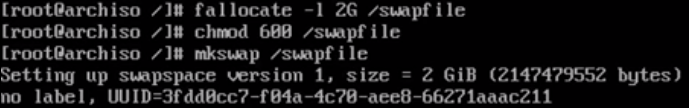
\includegraphics[width=0.7\textwidth]{./figures/swapfile.png}
  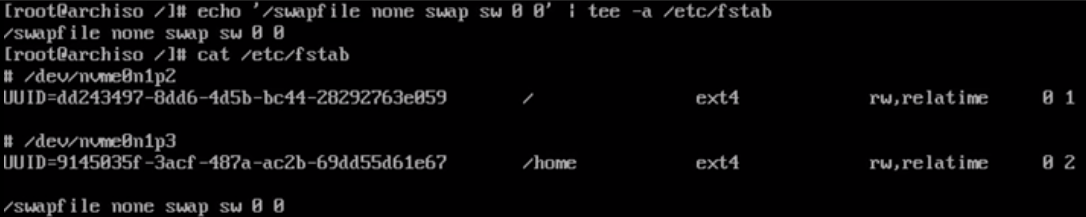
\includegraphics[width=\textwidth]{./figures/swapfile2.png}
\end{frame}

\begin{frame}[fragile]{Finish}
  \begin{itemize}
    \item \inlinebox{exit}, to exit out of chroot
    \item \inlinebox{umount -R /mnt}
      \item \inlinebox{umount -l /mnt} (to force unmount) or \inlinebox{umount -a}
    \item \inlinebox{poweroff} (not \inlinebox{reboot} to remove the iso from storage in virtualbox)
    \item in the UFEI firmware settings   choose the right bootloader for the esp on which the bootloader was installed (maybe secure boot has to be enabled for this) and give the esp with the bootloader the highest boot priority
  \end{itemize}
\end{frame}

\section{NixOs Base Installation}

\begin{frame}[fragile]{Dualbooting with Windows 11}
  \centering
  \begin{terminal}[minted language=nix]
    # boot.loader.systemd-boot.enable = true;
    boot.loader.efi.canTouchEfiVariables = true;
    boot.loader.grub.enable = true;
    boot.loader.grub.devices = [ "nodev" ];
    boot.loader.grub.efiSupport = true;
    boot.loader.grub.use0SProber = true;
  \end{terminal}
  \begin{itemize}
  \item \url{https://www.youtube.com/watch?v=82vrj22omyQ&list=PLXJMLVnWDKP0KQc1kbGbgyCz90yuecKKm&index=2&t=319s}
  \end{itemize}
\end{frame}

\begin{frame}[fragile]{Labeling}
  \begin{itemize}
    \item \inlinebox*{e2label /dev/XXX "new label"}
    \item \inlinebox*{swaplabel -L "new label" /dev/XXX}
    \item \inlinebox*{fatlabel /dev/XXX "new label"}
    \item \url{https://wiki.archlinux.org/title/Persistent_block_device_naming}
  \end{itemize}
\end{frame}

% \begin{frame}[fragile]{}{}
%   \begin{itemize}
%
%   \end{itemize}
% \end{frame}
